\documentclass[12pt, fleqn]{article}

\usepackage{../../../template/template}

 
\begin{document}

\begin{Task}[1 разбор задачи с кр]
    \[SL_2(\Z_3) \text{ и } S_4\]
    \[\text{Порядок 6 } \q \begin{pmatrix}
        2 & 1\\
        0 & 2
    \end{pmatrix} \begin{pmatrix}
        2 & 1\\
        0 & 2
    \end{pmatrix} = \begin{pmatrix}
        1 & 1\\
        0 & 1
    \end{pmatrix}\]
    \[\begin{pmatrix}
        1 & 1\\
        0 & 1
    \end{pmatrix} \begin{pmatrix}
        2 & 1\\
        0 & 2
    \end{pmatrix} = \begin{pmatrix}
        2 & 0\\
        0 & 2
    \end{pmatrix}\]
\end{Task}

\begin{Task}[2 разбор задачи с кр]
    %\[\abs{G} = pq\]
    %\[\ni x, y \qq \ord x = p \qq \ord y = q\]
    %\[\us{\text{порядок всех элементов}}{p, \ q \text{ или } pq}\]
    %\[x \mid \ord x = p\]
    %\[\abs{G/_{<x>} } = 1\]
    %\[y^q = x^l\]
    %\[y^p = e\]
\end{Task}

\section{Геометрия}
\begin{lect}{2019-11-08}
    \begin{Definition}
       \[X \text{ - линейное векторное пр-во над } \R\]
       \[\text{Тогда }  X \text{ - евклидово пр-во, если } \]
       \[\text{есть квадратичная линейная форма }
       <\cdot, \cdot> : \ X \times \X \to \R\]
       \begin{enumerate}
            \item $<ax + by, z> \ =\  a<x, z> + b<y, z>$
               \[a, b \in \R \q x, y, z \in X\]
            \item $<x, y> \ = \ <y, x>$
            \item $<x, x> \ \geq 0$
                \[<x, x> \ = 0 \ \rla \ x = 0\]
       \end{enumerate}
    \end{Definition}

    \begin{Definition}
        \[\abs{x} = \sqrt{<x, x>} \text{ - длина } x\]
        \[<x, y> \ = \arccos \left(\frac{<x, y>}{\abs{x} \cdot \abs{y}}\right)\]
        \[(x, y) = \abs{x}\abs{y} \cos (\angle\ x, y) \text{ скал произв.
        из геометрии}\]
    \end{Definition}

    \begin{Task}[7.1]
        \[u, v \q \abs{u}, \abs{v}, \angle \ u, v\]
        \begin{enumerate}
            \item $\angle \ $ между $x $ и $y$
            \item орт. проекцию $x$ на $y$
            \item $S_\triangle$ образ вект $x, y$
            \item центр и радиус окр., опис около около $\triangle$\\
                образ $x$ и $y$
            \item центр и радиус окр. впис в этот $\triangle$
        \end{enumerate}

        \[20)\]
        \[x = u  - 9v\]
        \[y = 7u + 5v\]
        \[\abs{u} = 2 \q \abs{v} = 3 \q \angle \ u, v = \frac{\pi}{3}\]
        \[<u, u>, \q <v, v>, \q <u, v>\]
        Нельзя просто перемножать координаты векторов!\\
        У нас не отонорм. базис
        \[<x, x>, \q <y, y>, \q <x, y>\]
        Воспользуемся линейностью
        \[<u - 9v, u - 9v> \ = \  <u, u - 9v> \ -\ <9v, u - 9v> = \]
        \[= \ <u, u> \ - \ <u, 9v> \ - \ <9v, u>  \ +\ <9v, 9v> = \]
        \[= \ <u, u> \ - \ 9 <u, v> \ - \ 9 <v, u>  \ +\ 81<v, v>\]
        \[4 - 18 \cdot 3 + 81 \cdot 9 = 679\]
        \[<7u + 5v, 7u + 5v> \ = \ 49<u, u>\ +\ 35 <u, v>\ +\ 35<v, u>\ +\
        25<v, v> = \]
        \[= 631\]
        \[<u-9v, 7u+5v> \ = \ 7<u, u>\ +\ 5 <u, v>\ -\ 63<v, u>\ -\ 45<v, v> = \]
        \[= -541\]

        \[\angle \ x, y = \arccos\left
        (\frac{-541}{\sqrt{631}\sqrt{679}}\right)\]

        Ищем орт. проекцию $x$ на $y$
        \begin{figure}[H]
            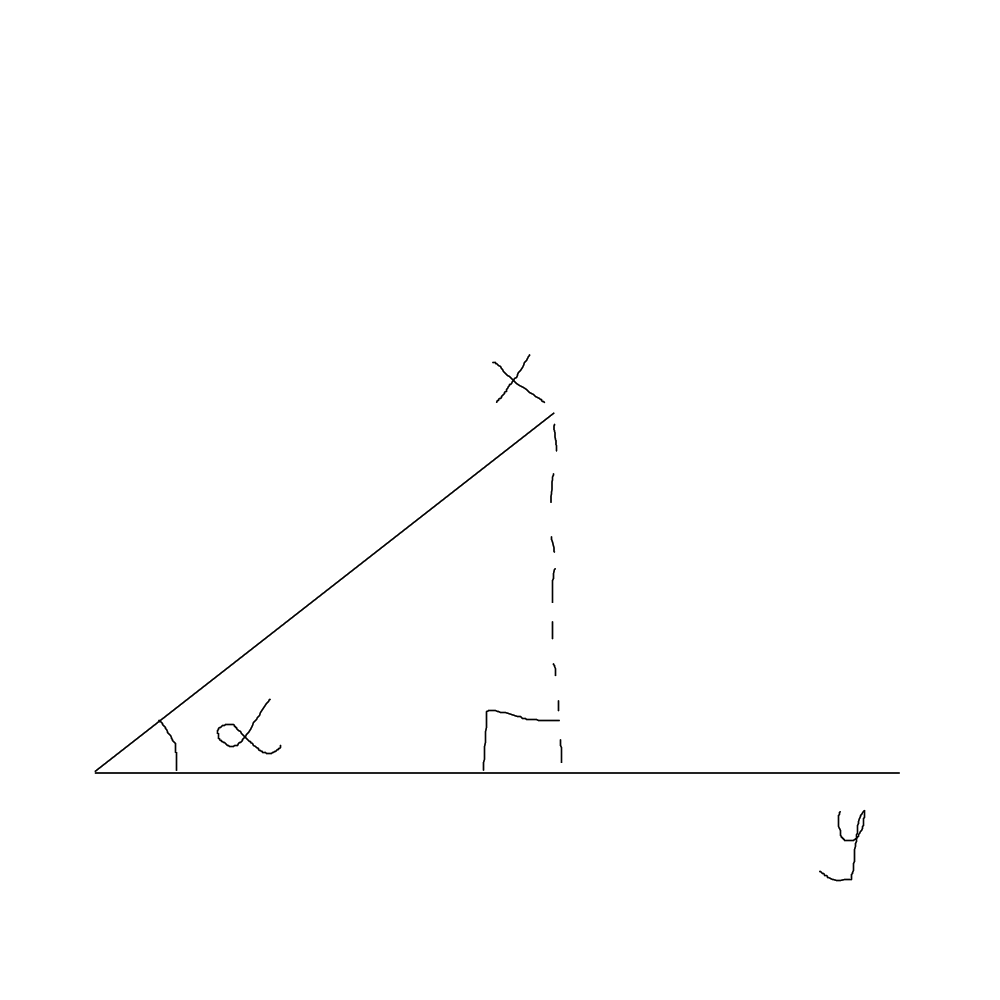
\includegraphics[width=7cm]{pics/1}
            \centering
        \end{figure}
        
        \[\frac{y}{\abs{y}}  \cdot \cos \alpha \abs{x} =  
        \frac{y}{\abs{y}} \frac{<x, y>}{\abs{x}\abs{y}}\abs{x}\]
        <<Подставить, все получить>>\\
        \\
        Найти площадь
        \begin{figure}[H]
            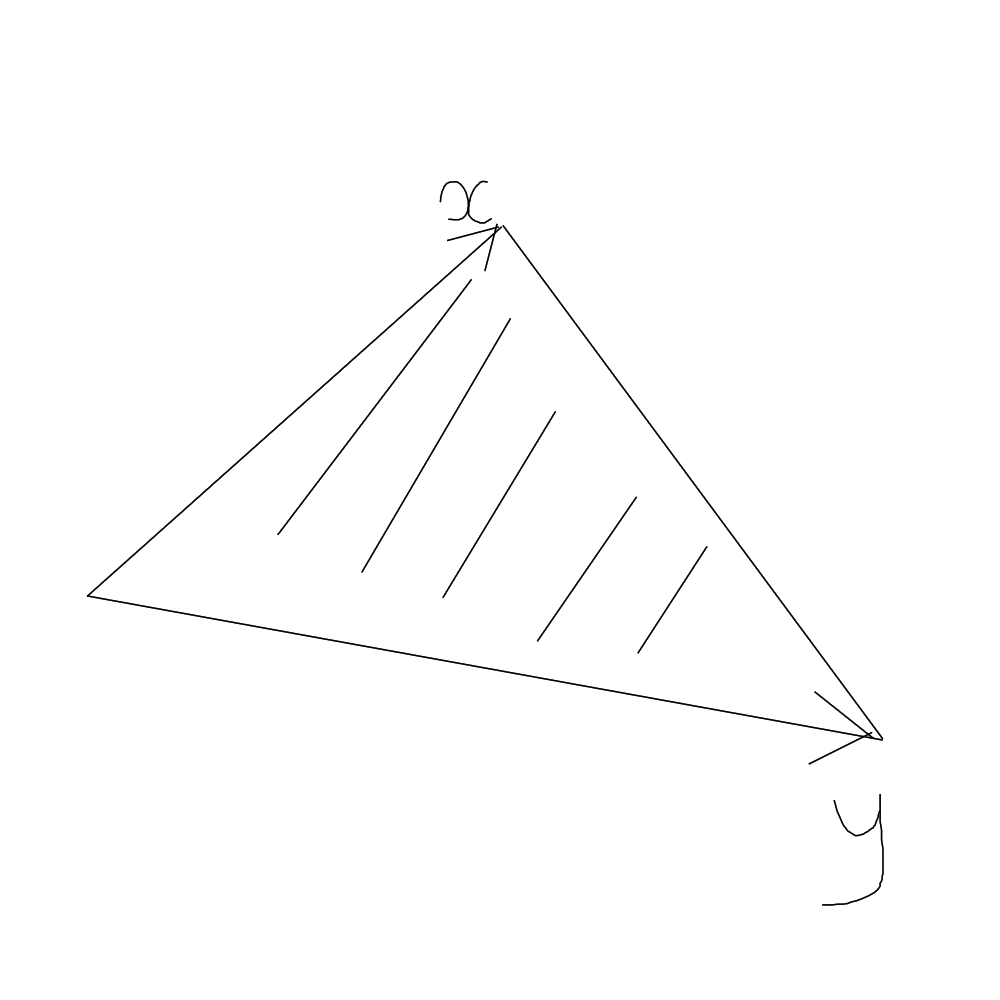
\includegraphics[width=7cm]{pics/2}
            \centering
        \end{figure}
        \[\frac{1}{2}\abs{x}\abs{y}\sin \alpha\]

        Ищем центр
        \begin{figure}[H]
            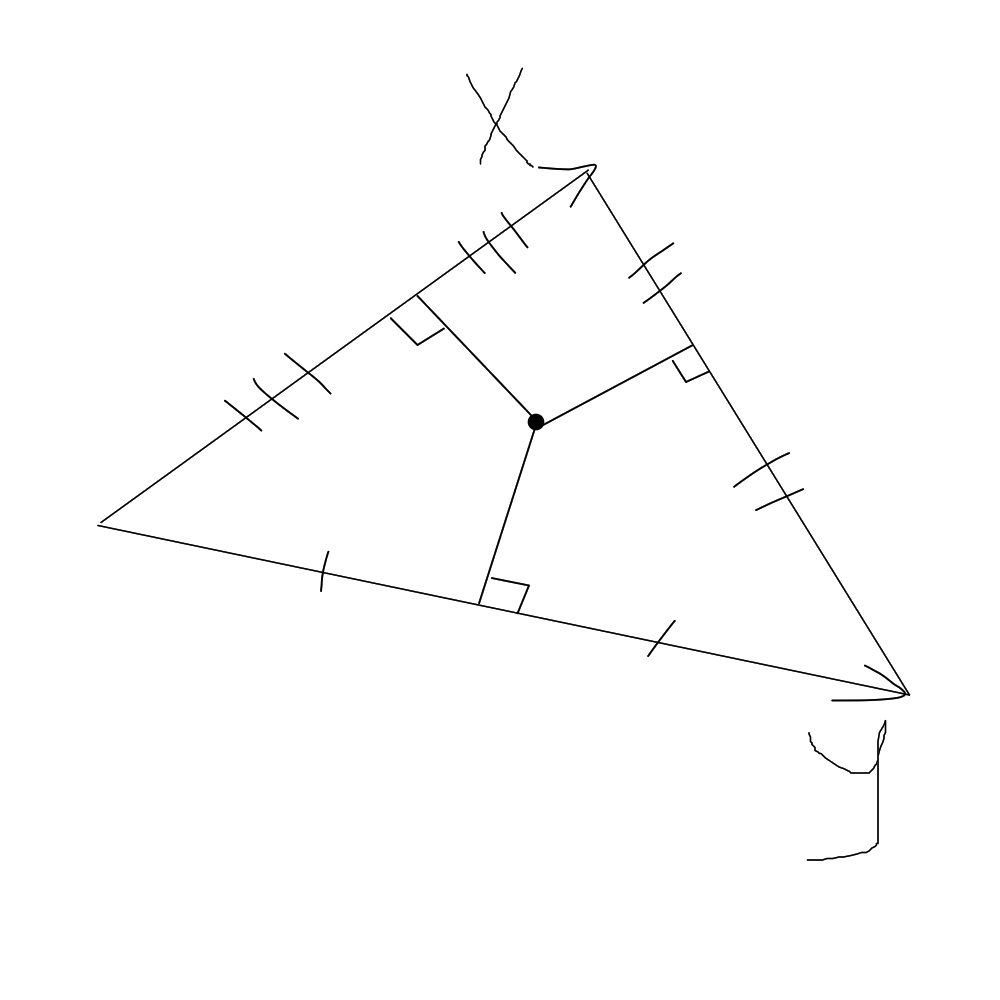
\includegraphics[width=7cm]{pics/3.png}
            \centering
        \end{figure}
        \begin{figure}[H]
            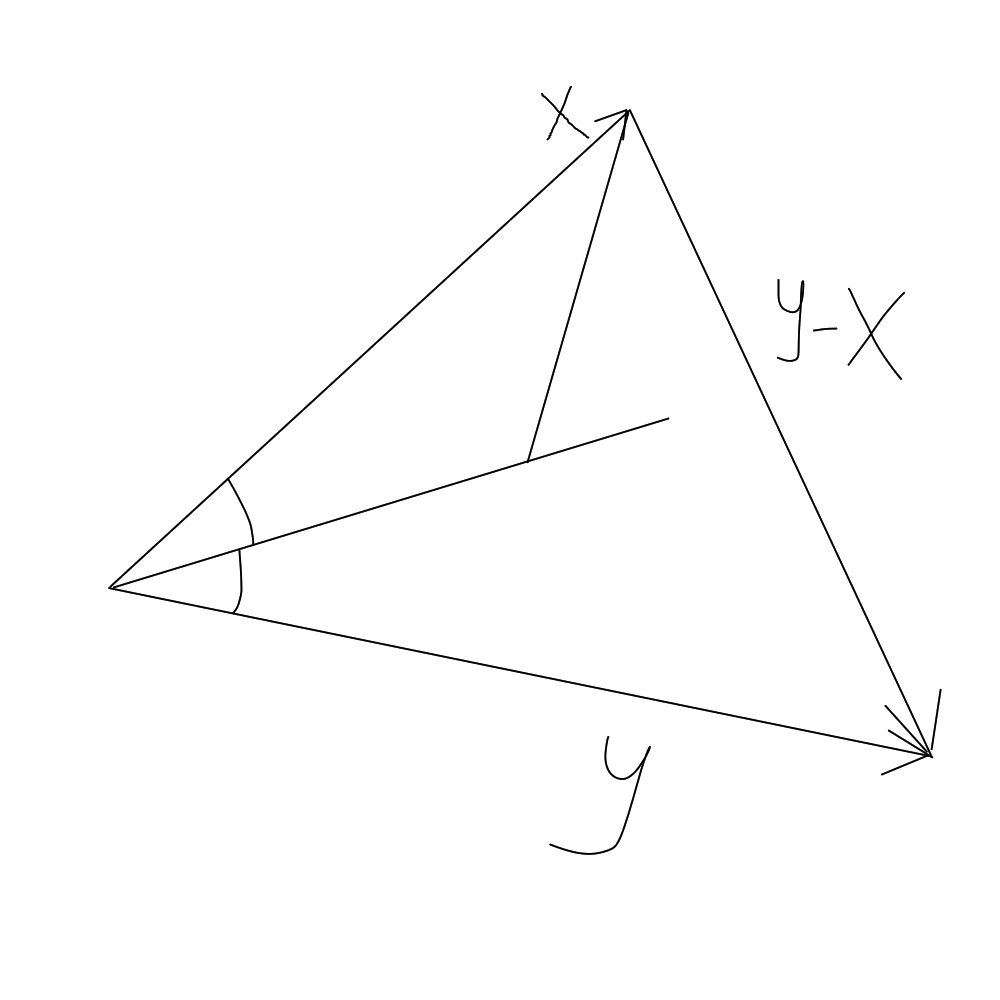
\includegraphics[width=7cm]{pics/4.png}
            \centering
        \end{figure}
        
        \[\frac{<x, ax + by>}{\abs{x}\abs{ax + by}} = 
        \frac{<y, ax + by>}{\abs{y}\abs{ax + by}}\]
        \[\frac{<ax + by - x, x>}{\abs{ax - by - x}\abs{x}} = 
        \frac{<ax - by - x, y - x>}{\abs{ax - by - x}{y - x}}\]
        \[r = \frac{S}{p}\]
        \[S \text{ - площадь}\]
        \[p \text{ - полуперим.}\]
        Дома сделать для описанной
    \end{Task}

    \begin{Task}[7.2]
        Найти угол между вектором и плоскостью в $\R^3$
        \[au + bv\]
        \begin{figure}[h]
            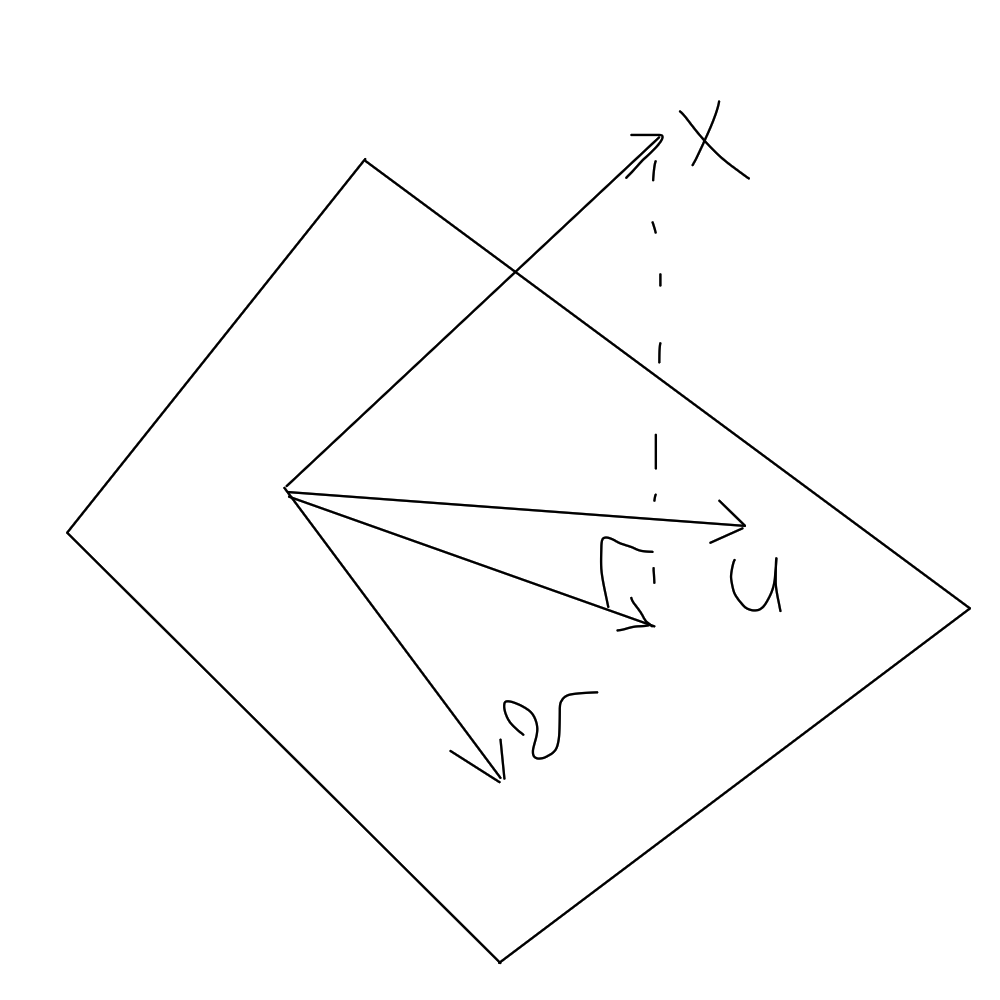
\includegraphics[width=7cm]{pics/5.png}
            \centering
        \end{figure}
        \[z \text{ - вектор между } u \text{ и } v\]
        \[z = au + bv\]
        \[(x - (au + bv), u) = 0\]
        \[(x - (au + bv), v) = 0\]
        \[<\begin{pmatrix}
            x_1 & x_2 & x_3 & x_4
        \end{pmatrix}, \begin{pmatrix}
            y_1 & y_2 & y_3 & y_4
        \end{pmatrix}> \ = x_1y_1 + x_2y_2 + x_3y_3 + x_4y_4\]
        \[(z - x) \perp \text{ пл-ти, порожд } u, v \rla \]
        \[\rla (z - x) \perp u \q (z - x) \perp v\]
        \[(z - x) \perp u \rla ((z - x), u) = 0\]
        \[(au + bv - x, u) = 0\]
    \end{Task}
\end{lect}

\end{document}
